\documentclass{article}

% Packages
\usepackage{amsmath} % For mathematical symbols and equations
\usepackage{graphicx} % For including images
\usepackage{cite} % For managing citations
\usepackage{lipsum} % For generating dummy text
\usepackage{algorithm} % For writing algorithms
\usepackage{algpseudocode} % For writing pseudocode
\usepackage{minted} % Syntax highlighting
\usepackage[a4paper, total={6in, 8in}]{geometry}
\usepackage{hyperref} % For hyperlinks


\title{Background Substitution Techniques on Human Segmentation Dataset}
\author{Abhishta Gatya Adyatma}
\date{March 2024}

\begin{document}

\maketitle

\begin{figure}[htbp]
    \centering
    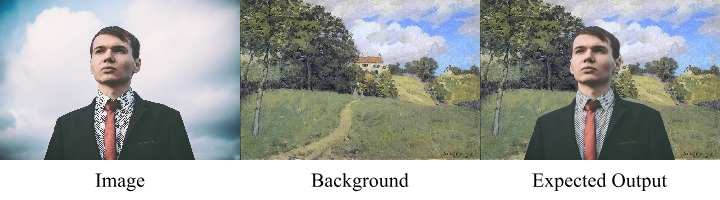
\includegraphics[width=0.9\linewidth]{img/Expect.jpg}
    \caption{Expected Result}
    \label{fig:problemi}
\end{figure}

\section{Introduction}

Background Substitution is a technique to extract a Foreground Object, whether a person, animal, or any object of interest to be displaced onto a new image seamlessly. Extracting the Foreground Object automatically and intelligently demands an increasingly complex algorithm depending on the subject of interest. Methods of extracting the Foreground Object typically rely on Image Segmentation techniques that aim to partition an image into multiple segments or regions based on certain characteristics, such as color, intensity, texture, or boundaries. This partition can be used to intelligently separate the Foreground Object and the Background to produce a mask (regions of interest within an image) and replace the Background with any image of choice.

At the core of this task, the author explores methods of Foreground Extraction that rely on Image Segmentation techniques particularly using Classical Methods \cite{ImageSegmentation2023}. The exploration will be focused on the method using Region Division and Graph Theory to build a mask of the Foreground Object. Evaluating the performance of each algorithm will use the Supervisely Persons Dataset \cite{SuperviselyPersons} that provides high-quality annotated person instances to use as the Foreground Object. These annotations will serve as the ground truth to compare with a generated mask of each algorithm experimented using the metric of Pixel Accuracy and Intersection over Union \cite{IoU}. Furthermore, the task is not complete without the process of image balancing, correcting, and mixing to explore a variety of options to seamlessly blend the Foreground Object with the newly adopted Background. This project will briefly discuss some methods and subjectively evaluate them as a side-by-side comparison.


\section{Dataset}

\begin{figure}[htbp]
    \centering
    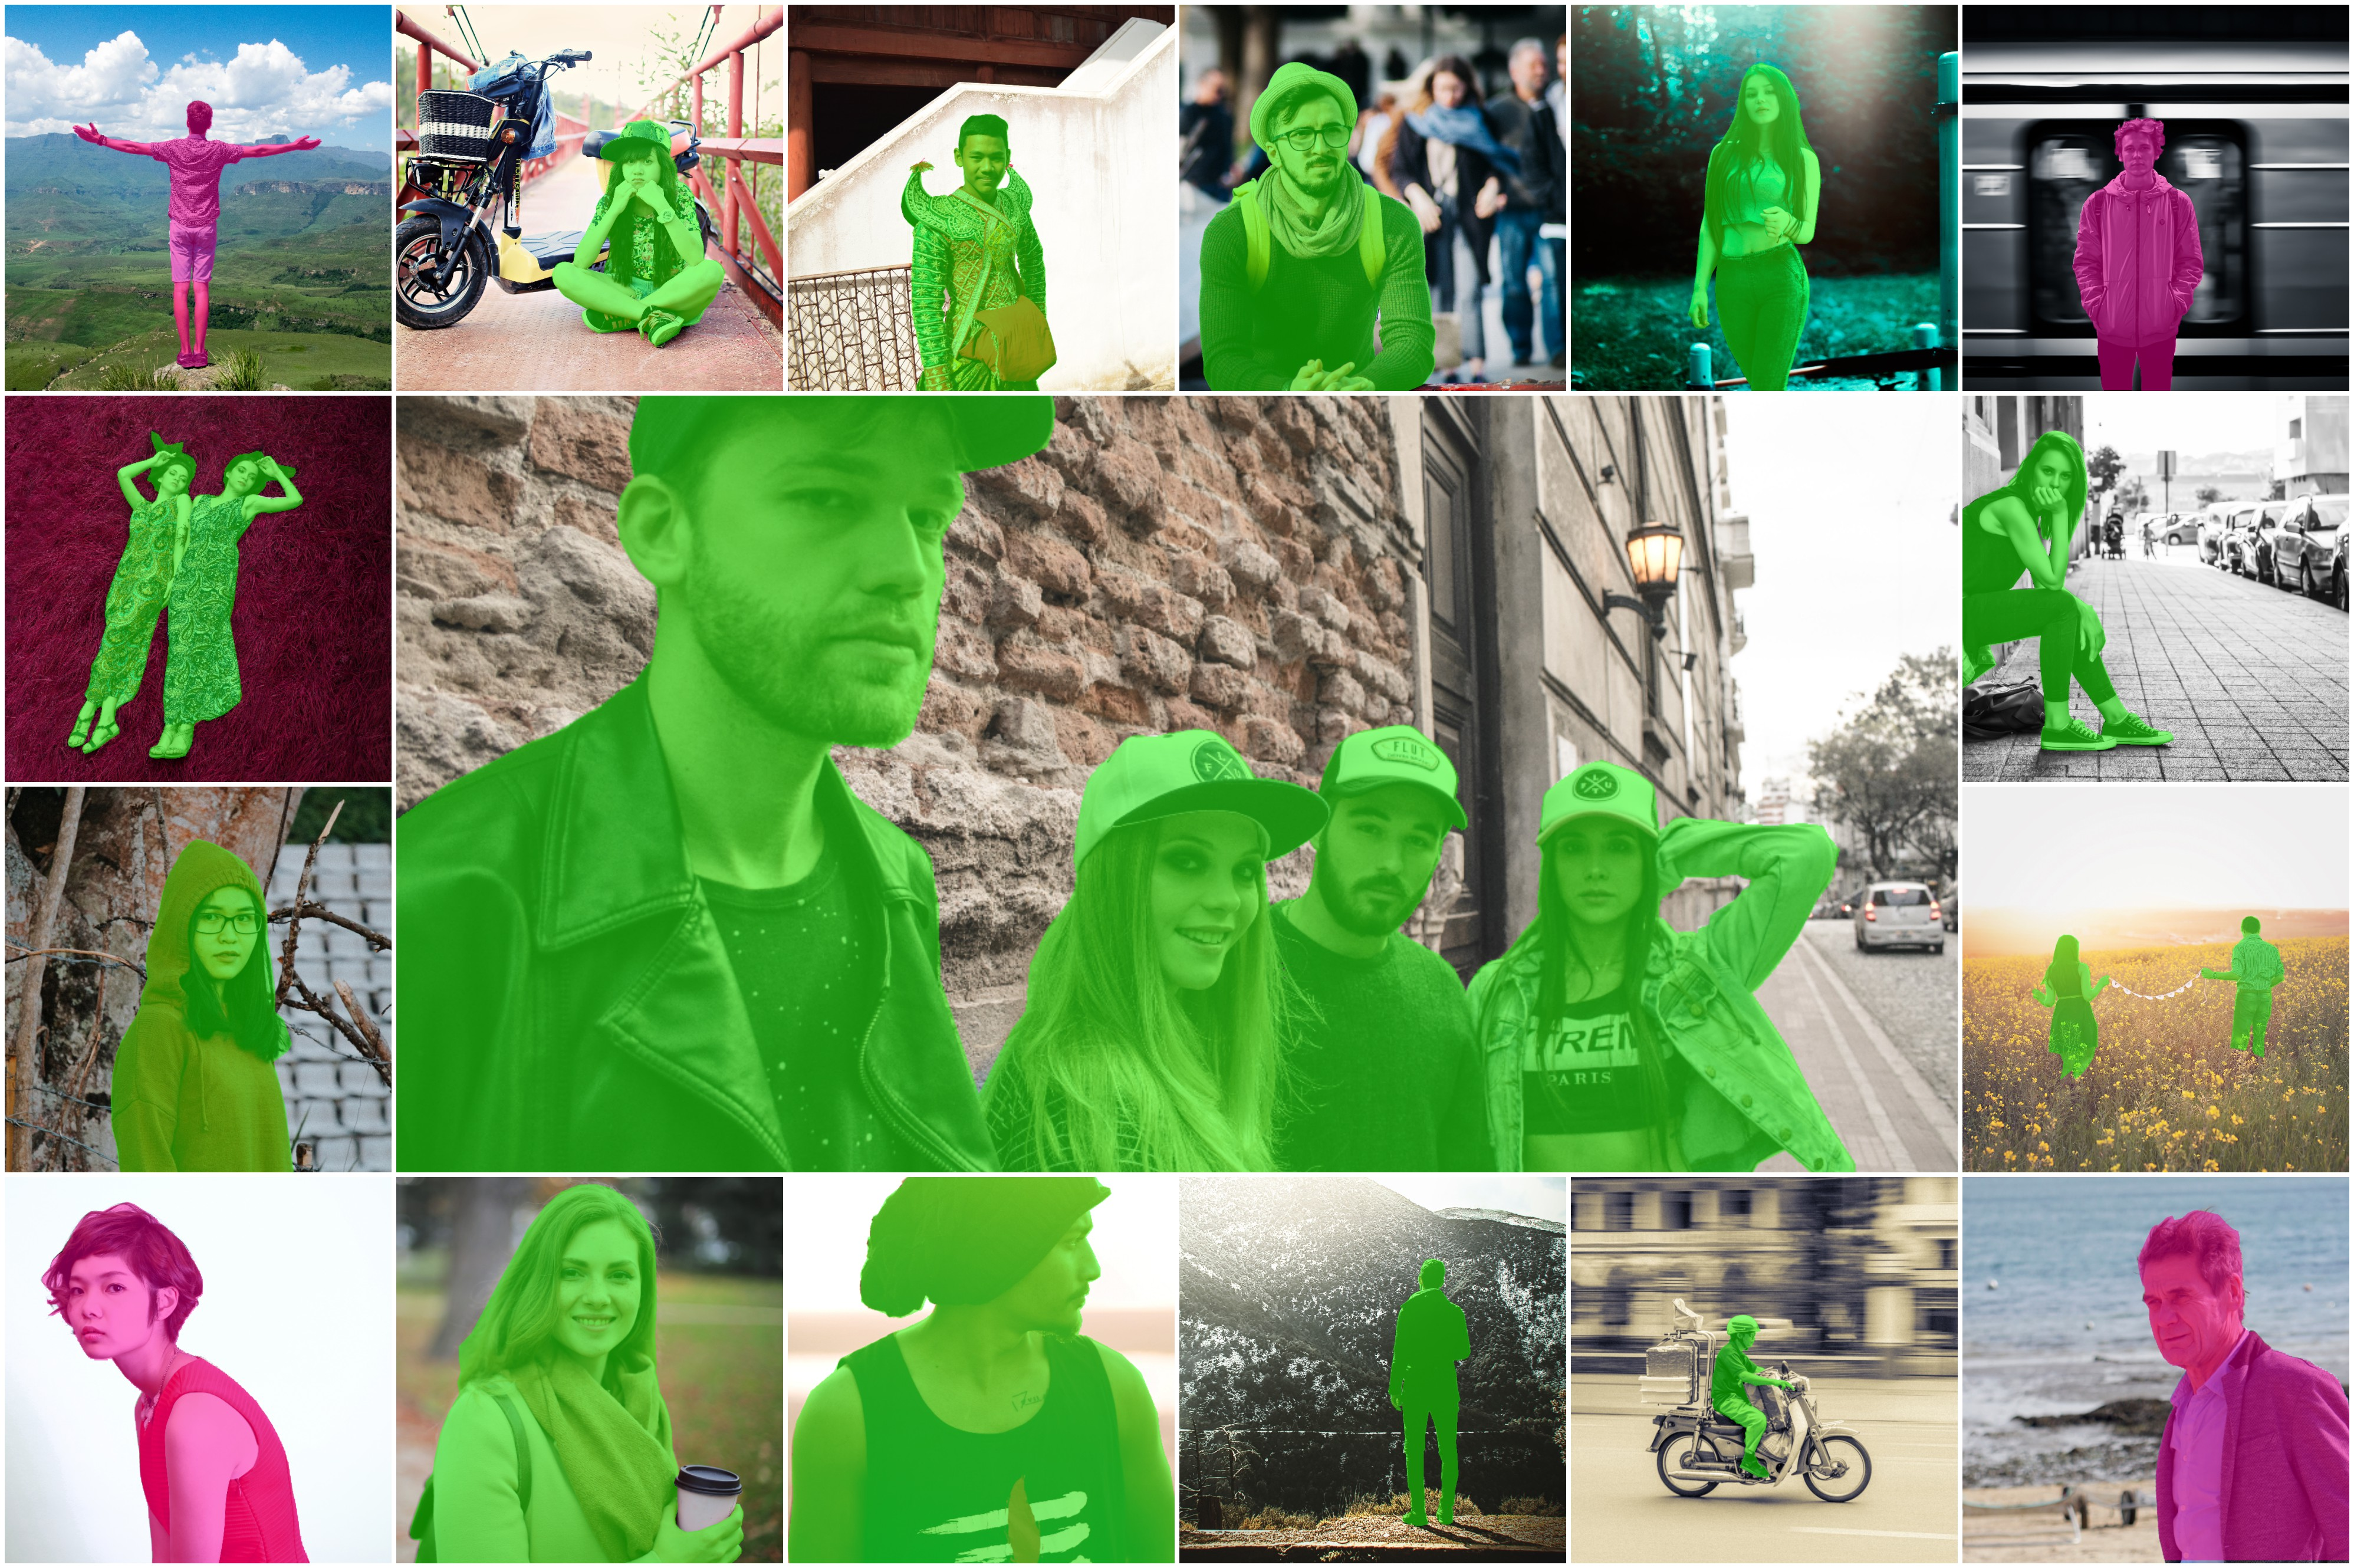
\includegraphics[width=0.6\linewidth]{img/Supervisely.jpg}
    \caption{Supervisely Human Segmentation (https://ecosystem.supervisely.com/projects/persons)}
    \label{fig:supervdb}
\end{figure}

Using the Supervisely Person Dataset \cite{SuperviselyPersons} enables this project to evaluate the generated mask of the algorithms (with a variety of parameters) by comparing it with the annotated person instance that the dataset provided. The sample version of this dataset comprises 2667 images each with an annotated instance of the image. These annotations are deemed to be detailed segmentation at the pixel level, which will serve as a great benchmark for evaluating this particular task. Notably, the image may contain more than one subject which will add complexity to the task.

For the Background substitute, arbitrarily it can be any image of choice. However, for this project, the author uses a collection of artwork from historical artists from the WikiArt Dataset (wikiart.org). The usage of this dataset as a Background Substitute is that artworks usually have different visual characteristics than photographs and are ideal for exploring various methods of blending options. Moreover, to uniform both datasets' image sizes, both datasets are resized to (720 $\times$ 400) dimensions.

\section{Algorithm}

This section will explore the algorithms to generate the mask using Image Segmentation techniques. The author concentrates on three algorithms based on Region Division and Graph Theory. These methods include Contour-based Morphological Segmentation, Watershed Segmentation \cite{Watershed2000}, and the GrabCut Algorithm \cite{Grabcut2004}.

\subsection{Contour-based Morphological Segmentation}

\renewcommand{\theFancyVerbLine}{
  \sffamily\textcolor[rgb]{0.5,0.5,0.5}{\scriptsize\arabic{FancyVerbLine}}}

This algorithm uses contour-finding techniques to identify the boundaries of the Foreground Object and apply morphological operations to perfect the identified boundaries as a usable mask to separate the Foreground Object and the Background. This implementation uses the Python snippet below.

\begin{minted}[mathescape,
               linenos,
               numbersep=5pt,
               gobble=2,
               frame=lines,
               framesep=2mm]{python}
    import cv2
    import numpy as np

    # Omitted Basic Setup (Loading Image, Resizing, Set Parameters)

    gray = cv2.cvtColor(image, cv2.COLOR_BGR2GRAY)
    _, thresh = cv2.threshold(gray, 0, 255, cv2.THRESH_BINARY | cv2.THRESH_OTSU)
    mask = np.zeros_like(gray)

    contours, _ = cv2.findContours(thresh, cv2.RETR_EXTERNAL, cv2.CHAIN_APPROX_SIMPLE)
    cv2.drawContours(mask, contours, -1, 255, thickness=cv2.FILLED)

    kernel = np.ones(kSize, np.uint8)
    fg_mask = cv2.morphologyEx(mask, cv2.MORPH_CLOSE, kernel)
\end{minted}

The process takes an image to be gray-scaled and thresholded (using the binary and adaptive methods) to be used for finding the contours of the Foreground Object. The method \textbf{cv2.findContours} identifies high-intensity pixels and searches for their neighbors iteratively to form an outline of the Foreground Object. This outline is drawn and filled onto the mask with the method \textbf{cv2.drawContours}. However, the mask is incomplete as many imperfections such as gaps and holes within the mask still reside. Fixing these imperfections using simple morphological operations to close these gaps and holes will improve the mask quality. Since morphological operations rely on a kernel, the author further explores how different kernel size may improve performance. In brief, the main idea of this algorithm takes a straightforward approach to identifying the Foreground Object and creating a boundary that approximates it.

\subsection{Watershed Segmentation}

This algorithm implements the Watershed Algorithm to segment the Foreground Object from the Background. The Watershed Algorithm takes advantage of gray-scaled image properties of efficiently identifying peaks (maxima) and valleys (minima) of an image to perform its process. It takes the intuition where it searches for isolated valleys (local minima) within the image and assigns a unique label covering the local minima. After each iteration, each covering the local minima of each frame of operation with labels, some of these minima may merge. To avoid this, it forms a boundary between the two regions while marking its location as it represents a potential segmentation boundary. This operation is complete when it reaches global maxima, leaving us with the segmentation boundary that has been created \cite{Watershed2000}. Below is the author's implementation.

\begin{minted}[mathescape,
               linenos,
               numbersep=5pt,
               gobble=2,
               frame=lines,
               framesep=2mm]{python}
    import cv2
    import numpy as np

    # Omitted Basic Setup (Loading Image, Resizing, Set Parameters)

    gray = cv2.cvtColor(image, cv2.COLOR_BGR2GRAY)
    _, thresh = cv2.threshold(gray, 0, 255, cv2.THRESH_BINARY_INV | cv2.THRESH_OTSU)

    kernel = np.ones(kSize, np.uint8)
    opening = cv2.morphologyEx(thresh, cv2.MORPH_OPEN, kernel, iterations=iterC)

    bg_area = cv2.dilate(opening, kernel, iterations=3)

    dist_transform = cv2.distanceTransform(opening, cv2.DIST_L2, 5)
    _, fg_area = cv2.threshold(dist_transform, 0.7 * dist_transform.max(), 255, 0)

    fg_area = np.uint8(fg_area)
    unknown = cv2.subtract(bg_area, fg_area)

    ret, markers = cv2.connectedComponents(fg_area)

    markers = markers + 1
    markers[unknown == 255] = 0
    markers = cv2.watershed(image, markers)

    fg_mask = np.where(markers == 1, 255, 0).astype('uint8')
\end{minted}

The initial idea of the Watershed Algorithm implementation is found to have an over-segmented result due to noise and any other image irregularities. Thus, the author implements a marker-based Watershed Algorithm which enables the author to specify which valley points should be merged and which should not, rendering it an interactive image segmentation technique.

In this approach, different labels are assigned to the known objects with the image. Specifically, regions identified as Foreground Objects of interest are labeled together and others with different labels. Any region in which certainty cannot be established is labeled uniformly, effectively serving as a marker. These markers are applied to use in the Watershed Algorithm as it updates the values of these labels. The result would display boundaries delineating the objects in the images are assigned a value uniquely which can be constructed as a mask.

In overview, the implementation applies a noise removal technique using morphological operations. Then, it identifies the Background Area and the Foreground Area with a labeled value of the distance between the two regions and threshold based on their value. After, it labels the connected component of the Foreground Area to prepare it for the Watershed Algorithm. Finally, the Watershed Algorithm processes the image with the given generated component label (marker) to segment the image based on it.

Since this implementation is interactive, a set of parameters can be adjusted to evaluate the implementation's performance and investigate the optimal parameter for this implementation. To scope the process of experimentation, the author limits the testing of parameters to the noise removal section through morphological operation by kernel size and iteration count. 

\subsection{GrabCut Algorithm}

GrabCut is an algorithm that leverages both graph theory and statistical properties of the image to perform image segmentation. It uses a technique known as Graph Cut, which transforms an image into a representation of a graph and partitions this graph into two disjoint sets by minimizing an energy function \cite{Grabcut2004}. This energy function captures both the similarity between adjacent pixels and the dissimilarity between the segmented regions and is combined with a Gaussian Mixture Model (GMM) to model the color distribution of the image regions to iteratively refine the segmentation between them. It updates these regions based on color and spatial proximity adjusting the probabilities of each pixel whether they belong to the foreground or background area. Below is the author's implementation of the algorithm using OpenCV.

\begin{minted}[mathescape,
               linenos,
               numbersep=5pt,
               gobble=2,
               frame=lines,
               framesep=2mm]{python}
    import cv2
    import numpy as np

    # Omitted Basic Setup (Loading Image, Resizing, Set Parameters)

    rect = (16, 16, 720, 400) # User-Estimate Bounding Box
    mask = np.zeros(image.shape[:2], np.uint8)

    bgdModel = np.zeros((1, 65), np.float64)
    fgdModel = np.zeros((1, 65), np.float64)

    cv2.grabCut(
        image,
        mask=mask,
        rect=rect,
        bgdModel=bgdModel,
        fgdModel=fgdModel,
        iterCount=iterC,
        mode=cv2.GC_INIT_WITH_RECT
    )

    fg_mask = np.where((mask == 2) | (mask == 0), 0, 255).astype('uint8')
\end{minted}

OpenCV's GrabCut implementation typically requires a user-specified bounding box, denoted as \textbf{rect}, to identify the likely Foreground and Background regions. This information will guide the algorithm's focus within the image and improve upon performance. However, since the information regarding the location of each object in the image is not provided within the dataset, the author opts for a standardized large bounding box (16, 16, 720, 400) covering a substantial portion of the image. This implementation will sacrifice slight performances of the algorithm however ensures that the comparison is fair across the aforementioned algorithms.

\section{Blending Method}

The task of background substitution also goes beyond displacing a Foreground Object onto a new Background, it also further explores the methods that will Blend the image onto the new Background to make the transition seamless. This seamless transition helps build the aesthetic of the final result to not seem like an edited or cutout image. Here, the author will explore a couple of blending methods, namely Color Balancing, Histogram Matching, and Gradient Mixing.

\subsection{Color Balancing}

Color Balancing is not typically used specifically to blend images, but rather to ensure consistency of colors across images. Color Balancing involves adjusting the colors of an image to achieve a desired look or correct any color casts caused by lighting conditions or other slight imperfections. However, in some cases, Color Balancing can indirectly aid in blending images by ensuring that the colors match more seamlessly between different parts of an image.

\begin{minted}[mathescape,
               linenos,
               numbersep=5pt,
               gobble=2,
               frame=lines,
               framesep=2mm]{python}
    import cv2
    import numpy as np

    # Omitted Basic Setup (Loading Image, Resizing, Set Parameters)
    # Omitted Generating Background Substitution Process
    
    lab_image = cv2.cvtColor(image, cv2.COLOR_BGR2LAB)
    l, a, b = cv2.split(lab_image)

    hist_l = cv2.calcHist([l], [0], None, [256], [0, 256])
    cdf_l = hist_l.cumsum() / hist_l.sum()
    mapped_l = np.interp(l.flatten(), np.arange(256), 255 * cdf_l).reshape(l.shape)

    low_bound = np.percentile(mapped_l, percent / 2)
    high_bound = np.percentile(mapped_l, 100 - percent / 2)
    clipped_l = np.clip(mapped_l, low_bound, high_bound)
    scaled_l = np.uint8(clipped_l)

    balanced_lab_image = cv2.merge((scaled_l, a, b))
    balanced_image = cv2.cvtColor(balanced_lab_image, cv2.COLOR_LAB2BGR)

\end{minted}

The above algorithm shows the implementation of the Color Balancing algorithm. It is done by first converting the image color space from BGR (Blue, Green, Red) to LAB (Lightness, Green-to-Magenta, Blue-to-Yellow) and splitting it into three different channels. Then it calculates the cumulative distribution function (CDF) of the L channel based on its histogram which will provide information about the cumulative probability distribution of pixel intensities in the L channel. Further, it maps the pixel intensities of the L channel to new values from the CDF to redistribute the pixel intensities in a way that enhances the contrast and brightness of the image. Finally, the author clips the values by a specific percentage so that the image will not be overexposed or underexposed and merges it back into the final result as a blended image. This technique is quite interactive as the percentage parameter can be tweaked to achieve a certain desired output. The effectiveness of this blending method will further be discussed within the results.

\subsection{Histogram Matching}

Histogram Matching is a technique to modify the histogram of an image to match a specified target histogram. It adjusts the pixel intensities of an image so that its histogram matches a desired distribution. Histogram Matching can be particularly useful for blending images when they have different lighting conditions, color casts, or exposure levels. By matching the histograms of the image, it can adjust its appearance to resemble the source or target more closely thus potentially blending the two images more seamlessly.

\begin{minted}[mathescape,
               linenos,
               numbersep=5pt,
               gobble=2,
               frame=lines,
               framesep=2mm]{python}
    import cv2
    import numpy as np

    # Omitted Basic Setup (Loading Image, Resizing, Set Parameters)
    # Omitted Generating Background Substitution Process

    source_lab = cv2.cvtColor(source, cv2.COLOR_BGR2LAB)
    target_lab = cv2.cvtColor(target, cv2.COLOR_BGR2LAB)

    source_l, source_a, source_b = cv2.split(source_lab)
    target_l, target_a, target_b = cv2.split(target_lab)

    def match_histograms(source, target):
        source_hist = cv2.calcHist([source], [0], None, [256], [0, 256])
        target_hist = cv2.calcHist([target], [0], None, [256], [0, 256])
    
        source_cdf = source_hist.cumsum() / source_hist.sum()
        target_cdf = target_hist.cumsum() / target_hist.sum()
    
        mapping = np.zeros(256, dtype=np.uint8)
        for i in range(256):
            mapping[i] = np.argmin(np.abs(source_cdf_norm - target_cdf_norm[i]))
    
        matched = mapping[source]
    
        return matched.astype('uint8')
    
    # Apply Function and Convert to BGR

\end{minted}

The algorithm above shows the matching algorithm on separate channels on the LAB color space. It involves calculating the cumulative distribution function (CDF) of the source and the target's histogram and mapping them to establish the correspondence between pixel intensities in the source and target images. For each intensity level, the closest intensity level in the source image that matches the target's CDF is determined. The implementation of this can take either the Foreground Image or the Background Image as the target, the desired output heavily depends on the user's decision of which image to use as the target for the blended image. 

\subsection{Gradient Mixing}

Gradient Mixing is an image blending technique that smoothly merges two images based on a gradient mask. This mask defines the blending strength at each pixel, allowing for precise control over the transition between the images. This method offers more precise control over the blending process to create that seamless transition that is desired.

\begin{minted}[mathescape,
               linenos,
               numbersep=5pt,
               gobble=2,
               frame=lines,
               framesep=2mm]{python}
    import cv2
    import numpy as np

    # Omitted Basic Setup (Loading Image, Resizing, Set Parameters)
    # Omitted Generating Background Substitution Process

    dimmed_mask = gradient_mask.copy()
    for i in range(iterC):
        dilated_mask = cv2.dilate(dimmed_mask, kernel, iterations=1)
        dilated_mask = cv2.multiply(dilated_mask, dimF)
        dimmed_mask = cv2.bitwise_or(dimmed_mask, dilated_mask)

    gradient_mask = dimmed_mask / 255.0
    inverted_mask = 1 - gradient_mask

    blended_image = np.zeros((720, 400, 3))

    blended_image[:, :, 0] = cv2.multiply(gradient_mask, foreground[:, :, 0]) + \
        cv2.multiply(inverted_mask, background[:, :, 0])
    blended_image[:, :, 1] = cv2.multiply(gradient_mask, foreground[:, :, 1]) + \
        cv2.multiply(inverted_mask, background[:, :, 1])
    blended_image[:, :, 2] = cv2.multiply(gradient_mask, foreground[:, :, 2]) + \
        cv2.multiply(inverted_mask, background[:, :, 2])

    blended_image = blended_image.astype(np.uint8)

\end{minted}

The above algorithm shows the implementation for Gradient Mixing with the addition of transforming the generated mask into a proper gradient mask that is usable for the mixing method. The mixing method works by having a gradient mask and an inverted mask from the mask that is generated by the Foreground Extraction process. The mix is a product of multiplying the foreground by the gradient mask and the addition of the background multiplied by the inverted mask. However, the generated mask from the Foreground Extraction process is not ideal to be used directly since the values are restricted to either 0 or 255, meaning the mixing process would not provide the gradual changes over the Foreground and the Background that is desired. The author uses a method to dilate the mask by some iteration and each dilated mask is multiplied by some factor to decrease the values gradually, making the mask have a gentler transition between the foreground area and the background area.

This method is ideally the best option for image blending as it is intuitive that a smoother transition of the mask may provide a smoother transition between the Foreground and the Background. This method is also interactive with adjusting the parameter for the dilation iteration and the dimming factor may contribute to different desired output.


\section{Result}

\subsection{Setup}

For this report's experimentation, the author analyzes the aforementioned algorithms using an Apple M1 Chip with 8 GB Memory. All algorithm implementations are using Python 3.9+ with OpenCV Python 4.9+. 
The evaluation is conducted by iterating the entire dataset with each model running with different parameters. Source code can be found at \href{https://github.com/abhishtagatya/backsub-cv}{Github : abhihtagatya/backsub-cv}

\subsection{Mask Generation}

\begin{figure}[htbp]
    \centering
    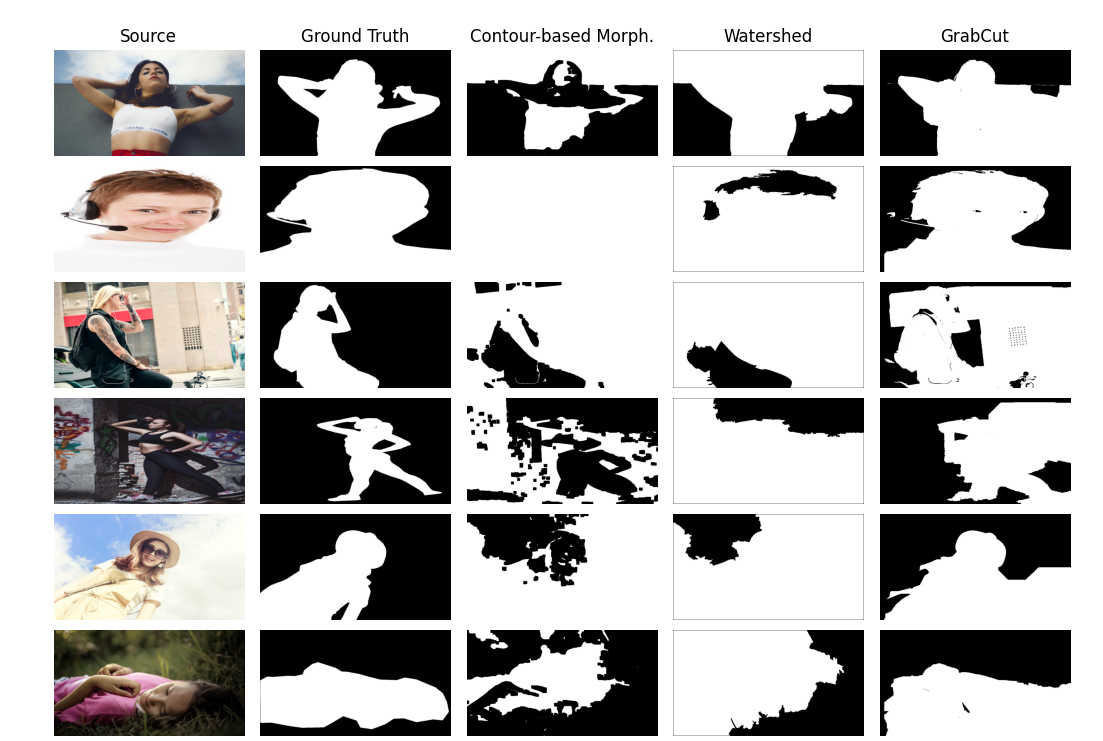
\includegraphics[width=1\linewidth]{img/MaskG.png}
    \caption{Sample of Generated Mask}
    \label{fig:gmask}
\end{figure}

The generation of a mask is the byproduct of any Image Segmentation algorithm that covers the area of the desired object of a given image. The quality of the generated mask determines the quality of the extracted Foreground Object to be displaced to the new Background, any imperfections could ruin the desired result quality for any Background Substitution task. Here, the author experimented on the aforementioned algorithms with different parameters to measure their performance over Time, Intersection-over-Union (IoU), and Pixel Accuracy shown in Table \ref{tab:maskg} and a sample of the mask generated by the algorithms side-by-side in Figure \ref{fig:gmask}.

\begin{table}
    \centering
    \begin{tabular}{|c|c|c|c|}
        \hline
         &  Time (ms) &  IoU&  Pixel Accuracy\\
         \hline
         CBMS-5x5   &  \textbf{1.53} &  0.2259  &  0.1544\\
         CBMS-7x7   &  1.62 &  0.2305  &  0.1588 \\
         CBMS-11x11 &  1.64 &  \textbf{0.2386}  &  \textbf{0.1667} \\
         \hline
         WS-2-5x5   &  \textbf{9.84} &  0.2893  &  0.2263\\
         WS-2-7x7   &  10.03 &  0.2902    &  0.2278\\
         WS-2-11x11 &  10.37 &  0.2897 &  0.2281 \\
         WS-3-5x5   &  9.86 &  0.2972   &  0.2363  \\
         WS-3-7x7   &  10.07 &  0.2984   &  0.2382 \\
         WS-3-11x11 &  10.29 &  \textbf{0.3011}  &  \textbf{0.2426} \\
         \hline
         GC-3   &  \textbf{1632.25} &  0.4991 &  \textcolor{red}{\textbf{0.2836}}  \\
         GC-4   &  1796.95 &  0.505  &  0.2816 \\
         GC-5   &  2021.95 &  \textcolor{red}{\textbf{0.5084}}  & 0.2803 \\
         \hline
    \end{tabular}
    \caption{Average IoU (Intersection-over-Union) and Pixel Accuracy. (1) CBMS-NxN: Contour-based Morphological Segmentation with (N x N) Kernel. (2) WS-R-NxN : Watershed Segmentation with R Iteration and (N x N) Kernel. (3) GC-R: GrabCut with R Iteration. \textcolor{red}{\textbf{Red}} indicates Best Result. \textbf{Bold} indicates Best in Method.}
    \label{tab:maskg}
\end{table}

The metric Intersection-over-Union (IoU) is used to evaluate the accuracy of object detection and segmentation tasks in computer vision. It measures the overlap between the predicted generated mask and the ground truth mask. Computing IoU is calculating the area of intersection between the predicted and ground truth regions and divided by the area of their union, generating a value ranging between 0 - 1 where higher values indicate better alignment between the two. Additionally, Pixel Accuracy compares the values between the generated mask and the ground truth mask whether they are equal or not. It provides pixel-wise precision between the generated mask and the ground truth mask indicating that higher values mean more accurate resemblance to the ground truth.

Table \ref{tab:maskg} shows the GrabCut algorithm outperforming the Watershed and the Contour-based Morphological Segmentation significantly, indicating that this algorithm produces a higher quality mask than the two. Generally, it is shown that using a higher value for the kernel or iteration opts for a better result. This is true for the case of the Watershed and Contour-based Morphological Segmentation where both use their parameters to remove noise whether in the image or the generated mask. However, the GrabCut algorithm performs worst in Pixel Accuracy as larger iterations are used. Additionally, the Time taken to generate the mask concerning the algorithm and its parameters gets increasingly longer, with GrabCut having the best result and taking the longest time to complete each segmentation. Thus, this table displays the advantages and drawbacks of all the algorithms mentioned and how sacrificing performance can achieve significantly faster segmentation completely depending on the use case in hand.

\subsection{Background Substitution Blending}

\begin{figure}[htbp]
    \centering
    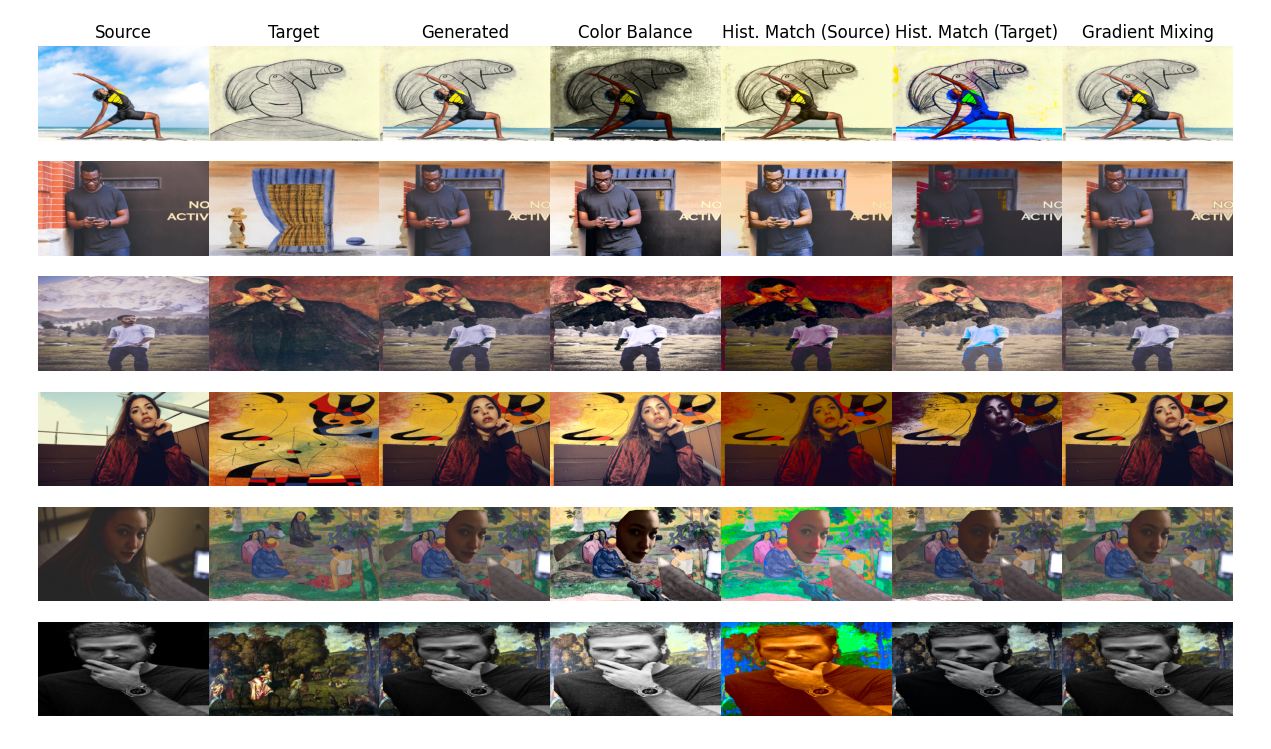
\includegraphics[width=1\linewidth]{img/GBlend.png}
    \caption{Blending Method of Background Substituted Images}
    \label{fig:bmimage}
\end{figure}

Figure \ref{fig:bmimage} shows all the implemented side-by-side from Color Balancing, Histogram Matching, and Gradient Mixing. The author chose the best method of Foreground Objection Extraction, which is the GrabCut algorithm to provide the mask and generate a Background Substituted image. From the Source and the Target, the author generates the first result without any Blending Method implemented. From these samples, it is already transparent that the Blending Method may improve or degrade the generated image.

Discussing the results of Color Balancing, some images may appear more seamlessly blended as a whole image rather than two separate images. However, this method may not always be the best solution changing the colors of the entire image may seem too edited when used incorrectly. Histogram Matching on the other hand has a uniquely different result to changing the colors than simple Color Balancing. By using a Source or Target image as a reference to match the generated output, some images improve the integration of the Foreground Object to the Background. However, not all cases benefit from this technique as some appear darker since the Source and Target images have drastically different histogram distributions.

One of the techniques that appears consistent throughout this sample is the Gradient Mixing method as it improves the images slightly around the colliding region of the Foreground and Background rather than the entire image as a whole. The effect is faint, yet also when looked closely the gradual changes of the regions seem to blend the image better than just plain displacement.

These methods show that Blending Methods are crucial for Background Substitution tasks and what methods to use depends on the desired aesthetic and pairs of images. However, this experiment can conclude that Gradient Mixing is a safe option as the effect of improvement is slight rather to other methods mentioned. A remark regarding these methods is that users of this algorithm may combine methods to achieve their desired look.

\section{Conclusion}

This project has experimented with Background Substitution methods from Foreground Object Extraction through Image Segmentation and Blending Methods to improve the aesthetic of the Foreground Object displacement. While the achievement of the GrabCut algorithm has proved to be superior within this report, recent methods of Machine Learning and Deep Learning have uplifted the quality of generating masks for more complex objects than the aforementioned methods. However, it is to be noted that Classical Methods and simple Blending Methods still hold an advantage over time, as the author was able to achieve a reasonably low-resolution Time for each image, something that might not quite be achievable yet with modern heavy Machine Learning and Deep Learning methods. Regardless, the project successfully implemented a variety of options to use for the Background Substitution task and demonstrated the capability of each method.

\bibliographystyle{plain} % Choose a style
\bibliography{references} % Assuming your file is named 'references.bib'

\end{document}
